\documentclass{article}
\usepackage{hyperref}
\usepackage{amsmath}
\usepackage{amsfonts}
\usepackage{amssymb}
\usepackage{graphicx}\graphicspath{{figs}{.}}
% \usepackage[margin=1in]{geometry}
\usepackage{comment}

\title{Denoising in (Electron?) Microscopy 3D Imaging}

\author{Vicente González-Ruiz and José Jesús Fernández Rodríguez}

\begin{document}
\maketitle

\begin{abstract}
  We compare several 3D image denoising algoritms in the field of
  electron microscopy of biological specimens. Microscopy images are
  characterized by a very low SNR and therefore, denoising algorithms
  are required to improve their posterior analysis. It is also common
  that there exist only one noisy version of the images, which
  increases the dificulty of an objective comparison of the algorithms
  (we don't have a ground truth to compare with). For this reason, one
  only can estimate the quality of the denoised images perceptually or
  alternatively, considering prior known image features such as the
  maximum resolution of the miscroscope.
\end{abstract}

\tableofcontents

\section{Common sources of noise in microscopy imaging}

In microscopy, there are three main sources of noise: (1)
\emph{dark noise} which corresponds to the electronic noise generated
by the thermal agitation of electrons, (2) \emph{photon noise} (or
shot noise) that is generated from the statistical fluctuations of the
number of photons sensed at a given signal exposure level, and (3) the
\emph{readout noise}, generated by the non-perfectness of the output
electronic amplifier using in the process of converting photon or
electron accumulations into voltages. Therefore, the level of noise
depends on the exposure time, experimental conditions affecting the
sensors such as the temperature, or other parameters like the
fluorescence of the structures. Dark and photon noises follow a Poisson
distribution $\mathcal{P}(\lambda)$, where $\lambda$ represents the
average dark flux. Readout noise is modeled as zero-mean additive
white Gaussian noise \cite{meiniel2018denoising,zhou2020wirtinger}.

\begin{comment}
\subsection{Quantization noise}
All digital capturing devices generate quantization noise which is
usually modeled as additive zero-mean uniform noise
(${\mathbf N}\sim{\mathcal U}(c)$). The PDF (Probability Density
Function) is defined by
\begin{equation}
  f(x; c) = \Pr({\mathbf N}^{(i)}_j{=}x) \triangleq \begin{cases}
    \frac{1}{2c} & \text{for } -c \le x \le c, \\[8pt]
    0 & \text{for } x < c \ \text{ or } \ x > -c,
  \end{cases}
\end{equation}
$x$ and $f$ continuous, where $\Pr(\cdot)$ represents the
probability of $\cdot$, and $c$ controls the amplitude of the
noise. Notice that in this case, $\overline{\mathbf{N}}^{(i)}=0$ and
therefore, $\overline{\mathbf N}={\mathbf 0}$ (see
Eq.~\ref{eq:noise_expectation_2}). 
\end{comment}

\subsection{Additive white Gaussian (AWG) noise}
A noisy image $\hat{\mathbf X}$ corrupted by AWG noise is modeled as
\begin{equation}
  \hat{\mathbf X} = {\mathbf X} + {\mathbf N},
  \label{eq:AWG_noise_model}  
\end{equation}
where $\mathbf{X}$ is the \emph{clean image} (without noise, ground
truth usually unknown) with a $J$ pixels (or voxels in
the 3D case), and ${\mathbf N}\in\mathbb{R}^J$ is a tensor of random
samples. In the case of AWG,
${\mathbf N}\sim{\mathcal N}(\mu=0,\sigma^2)$, with PDF (probability
density function)
\begin{equation}
  \Pr({\mathbf N}_j{=}x) = \frac 1 {\sigma\sqrt{2\pi}} e^{-\frac{x^2}{2\sigma^2} },
\end{equation}
$x\in\mathbb{R}$ continuous (in our context, the value of a
pixel/voxel), representing $\mu$ the mean and $\sigma$ the standard
deviation of the noise. Notice that this model is signal-independent
because nothing can said about ${\mathbf N}$ known $\hat{\mathbf X}$
(except that both have the same shape and size $J$).

By definition, the spectrum of AWG noise is flat. Therefore, the
performance of a pure low-pass filter denoiser will depend on the
shape of the spectrum of $\mathbf{X}$.

\subsection{Poisson noise}
Poisson noise is defined by the PMD (Probability Mass
Distribution)\footnote{Also called discrete PDF.}
\begin{equation}
  \Pr({\mathbf N}_j{=}k) = \frac{\mathbf{\lambda}_j^ke^{-\mathbf{\lambda}_j}}{k!},
  \label{eq:PN}
\end{equation}
which describes the probability of $k\in\mathbb{N}$ events ocurring
within an observed interval (of time, for example), when, in average
we have ${\mathbf \lambda}_j\in\mathbb{R}$ events in such interval.

In this case, we model the noisy signal as
\begin{equation}
  \hat{{\mathbf X}}_j = \frac{{\mathbf X}_j^{k} e^{-{\mathbf X}_j}}{k!}.
\end{equation}

As it can be seen, this is a signal-dependent model because the
brighter parts of $\hat{\mathbf X}$ will have a higher mean value and
a higher variance\footnote{The mean and variance of a Poisson law are
  both equal to $\lambda$.}, and therefore higher noise level (and
viceversa) \cite{meiniel2018denoising}. When necessary, we will
highlight this by writting ${\mathbf N}({\mathbf X})$.

Poisson noise is generated based on the intensity of the underlying
signal and therefore, the frequency characteristics of Poisson noise
resemble the spectrum of the clean signal.

\subsection{Mixed Poisson-Gaussian noise}
A more realistic noise model in microscopy consists in a combination
of both Poisson and AWG noise, which is commonly called mixed
Poisson-Gaussian (MPG) noise \cite{meiniel2018denoising}. In this
case, we have that
\begin{equation}
  \Pr({\mathbf N}_j{=}k) = \frac{e^{-\lambda_j}}{\sigma\sqrt{2\pi}}\sum_{p=0}^{\infty}\frac{\lambda_j^p}{p!} e^{-\frac{\gamma p - k}{2\sigma^2}},
  \label{eq:PN}
\end{equation}
where
\begin{equation}
  \hat{\mathbf X} = {\mathbf N}_{\mathrm{Gaussian}} + \gamma{\mathbf N}_{\mathrm{Poisson}}({\mathbf X}).
  \label{eq:MPG_noise_model} 
\end{equation}
Therefore, MPG noise is signal-dependent and it's spectrum depends on the clean image $\mathbf{X}$.

% \subsection{Speckle noise}
% Speckle noise is generated in optical devices that use coherent light sources (lasers), such as in fluorescence microscopy \cite{kumar2021speckle}. Speckle noise is signal-dependent, so its variance changes with the intensity of the true image. It has been modeled as zero-mean multiplicative Gaussian noise \cite{} and as Rice noise \cite{}.

% Multiplicative zero-mean Gaussian noise, modeled as
%   \begin{equation}
%     \hat{\mathbf X}^{(i)} = {\mathbf X} (1 + {\mathbf N}^{(i)}),
%     \label{eq:MGN}
%   \end{equation}
%   where ${\mathbf N}\sim{\mathcal N}(\mu,\sigma)$. This is a signal-dependent noise present
%   in synthetic aperture radar (SAR) and ultrasound images is usually
%   considered speckle noise.
  
%   Another distribution used for modeling speckle noise is the Rice
%   distribution ($\mathbf{N}\sim\mathrm{Rice}(\nu,\sigma)$), with PDF
%   \begin{equation}
%     f(x; \nu,\sigma) = \Pr({\mathbf N}^{(i)}_j{=}x) = \frac{x}{\sigma^2}e^{\frac{-(x^2+\nu^2)}{2\sigma^2}}I_0\left(\frac{x\nu}{\sigma^2}\right),
%   \end{equation}
%   where $x$ is continuous, and $I_o$ is the modified Bessel function
%   of the first kind with order zero. Rician noisy tensor instances can
%   be generated with
%   \begin{equation}
%     \hat{\mathbf X}^{(i)} = \sqrt{ ({\mathbf X} + {\mathbf N}_{\text{real}}^{(i)})^2 + ({\mathbf N}_{\text{imag}}^{(i)})^2}.
%   \end{equation}
%   %Notice that the Rayleigh distribution ($\mathbf{N}\sim\mathrm{Rayleigh}(\sigma)$),
%   %which is defined by the PDF
%   %\begin{equation}
%   %  {\mathbf N}^{(i)} \sim f(x; \sigma) = \frac{x}{\sigma^2} e^{-x^2/(2\sigma^2)}, \quad x \geq 0,
%   %\end{equation}
%   %continuous both, $x$ and $\sigma$ (the scale parameter) is a
%   %particular case of Rice distribution when $\nu=0$.
%   Notice that, even being $\nu=0$ (in whose case we are working with
%   the Rayleigh distribution
%   ($\mathbf{N}\sim\mathrm{Rayleigh}(\sigma)$)), the mean of the noise
%   is not zero. The noise that corrupts magnetic resonance images is
%   usually modeled as Rician/Rayleigh noise.

% \subsection{Shot noise}

% \section{Noise models}
% \label{sec:noise_models}

% Let $\mathbf{X}$ be a \emph{clean signal} (without noise, ground truth
% usually unknown) tensor, and $\hat{\mathbf X}^{(i)}$ the $i$-th
% noisy-version tensor random instance of $\mathbf{X}$ generated, in
% general, through
% \begin{equation}
%   \hat{\mathbf X}^{(i)} = f(\mathbf{X}, \mathbf{N}^{(i)}),
%   \label{eq:general_model}
% \end{equation}
% where ${\mathbf N}^{(i)}$ an $i$-th (unknown) noise tensor instance
% with the same shape as $\mathbf{X}$.

% We assume that ${\mathbf X}$ and $\mathbf{N}$ are statistically
% independent, and therefore, nothing can be said about
% ${\mathbf N}^{(i)}$ if we know $\hat{\mathbf X}^{(i)}$, and
% viceversa, and therefore, it is impossible to obtain ${\mathbf X}$
% from a single $\hat{\mathbf X}^{(i)}$.

% \subsection{Signal-independent noise model}
% In SIN (signal-independent noise) models, the noise is statistically i.i.d. (independent and
% identically distributed), i.e., the random values of ${\mathbf N}^{(i)}$ satisfy that
% \begin{equation}
%   {\mathbb E}[\{{\mathbf N}^{(i)}_j\}_{j=1}^J]=\frac{1}{J} \sum_{i=1}^J {\mathbf N}_j^{(i)}=\overline{\mathbf N}^{(i)},
%   \label{eq:noise_expectation_1}
% \end{equation}
% where ${\mathbf N}^{(i)}_j$ is the $j$-th (scalar) value
% of ${\mathbf N}^{(i)}$, and
% \begin{equation}
%   J=\prod_{k=1}^D \mathbf{X}.\text{shape}[k],
% \end{equation}
% being $D$ the number of dimensions of the signal (in microscopy, usually 2 or 3).

% SIN models are also called additive noise models defined by
% \begin{equation}
%   \hat{\mathbf X}^{(i)} = {\mathbf X} + {\mathbf N}^{(i)}.
%   \label{eq:additive_noisy_model}
% \end{equation}

% \subsection{Signal-dependent noise (SDN) models}
% In SDN models, the amplitude of the random noise samples depends on
% the clean signal (see Eq.~\ref{eq:general_model}).

% %\begin{equation}
% %  \hat{\mathbf X}^{(i)} = \mathbf{X} + {\mathbf N}^{(i)}(\mathbf{X}),
% %  \label{eq:SDN_model}
% %\end{equation}
  
\section{Distortion metrics}

\subsection{\href{https://en.wikipedia.org/wiki/Root_mean_square_deviation}{RMSE (Root Mean
    Square Error)}}

Having two tensors $\mathbf{X}$ and $\mathbf{Y}$ of size $J$,
\begin{equation}
  \text{RMSE}(\mathbf{X},\mathbf{Y}) \triangleq \sqrt{\frac{1}{J}\sum_{i=1}^J(\mathbf{X}_i - \mathbf{Y}_i)^2}.
\end{equation}
Notice that the RMSE expresses the distortion in the same units as the
samples.

\subsection{\href{https://en.wikipedia.org/wiki/Structural_similarity_index_measure}{SSIM
    (Structural Similarity Index Measure)}}
The SSIM try to model the human perception of the differences between
two images $\mathbf{X}$ and $\mathbf{Y}$. The metric returns a real
number between $[-1, 1]$, $-1$ representing the perfect dis-similarity
case, $0$ no similarity, and $1$ perfect similarity. The SSIM index is
determined (splitting input images into $M$ non-overlapping blocks)
with
\begin{equation}
  \text{SSIM}(\mathbf{X}, \mathbf{Y}) \triangleq \frac{1}{J} \sum_{j=1}^J \frac{(2\overline{\mathbf{x}}_j \overline{\mathbf{y}}_j + c_1)(2\sigma_{\mathbf{x}_j \mathbf{y}_j} + c_2)}{(\overline{\mathbf{x}_j^2} + \overline{\mathbf{y}_j^2} + c_1)(\sigma^2_{\mathbf{x}_j} + \sigma^2_{\mathbf{y}_j} + c_2)},
\end{equation}
where $\overline{\mathbf x}_j$ is the mean of the $j$-th block of
$\mathbf{X}$, $\sigma^2_{\mathbf{x}_j}$ is its variance (equivalently
for $\mathbf{Y}$), $\sigma_{\mathbf{x}_j\mathbf{y}_j}$ is the
covariance of both blocks, $c_1=(k_1L)^2$, $c_2=(k_2L)^2$ are two
variables used to stabilize the division with weak denominator, $L$ is
the dynamic range of the voxel values, with constants with default
vales $K_1=0.01$, and $k_2=0.03$, and where the default size of the
local blocks is $7^D$, where $D$ is the number of dimensions ($D=2$
for images and $D=3$ for volumes). When comparing images (or volumes),
values below $0$ does not make sense.

\subsection{\href{https://en.wikipedia.org/wiki/Pearson_correlation_coefficient}{PPC
    (Pearson Correlation Coefficient)}}
The PPC is given
by
\begin{equation}
  \text{PPC}(\mathbf{X}, \mathbf{Y}) := \frac{\sum_j(\mathbf{X}_j - \overline{\mathbf{X}})(\mathbf{Y}_j - \overline{\mathbf{Y}})}{\sqrt{\sum_j (\mathbf{X}_j - \overline{\mathbf{X}})^2 \sum_j (\mathbf{Y}_j - \overline{\mathbf{Y}})^2}},
\end{equation}
and measures the linear correlation between two tensors $\mathbf{X}$
and $\mathbf{Y}$.  As happen with the SSIM, the output is in
$[-1, -1]$, meaning $-1$ a perfect negative linear relationship
between the input tensors, $0$ no linear relation, and $1$ a perfect
coincidence. However, as happens with the SSIM, in microscopy values
below $0$ never should occur.

\subsection{FSC (Fourier Shell Correlation) curve}
The FSC curve measures the similarity between two 3D volumes
represented in the Fourier domain \cite{verbeke2024self} (for the 2D
case, the equivalent metric is called FSC (Fourier Ring
Correlation)). Each point of the curve prepresents the correlation
between two ``shells'' (``rings'') of Fourier coefficients of both
volumes (images).

An advantage of the FSC over other similarity metrics such as the
RMSE, the SSIM and the PPC is that FSC values depend on the frequency,
and this can be interesting in some scenarios, such as microscopy,
where the resolution of the microscope is finite and known a priori
\cite{nieuwenhuizen2013measuring}. Notice that, with this information,
we can know whether the denoising is removing the high-frequency
components of the clean signal, or on the contrary, basically
noise. For this reason, in some fields such as single particle
electron cryo-microscopy (cryo-EM), the FSC curve has become the
universal resolution metric and is used to assess the quality of 3D
reconstructions \cite{rosenthal2003optimal,scheres2012prevention}.

A FSC value of the FSC curve is determined by~\cite{verbeke2024self}
\begin{equation}
\text{FSC}(\mathbf{X}, \mathbf{Y}; r) := \frac{\sum_{i \in S_r} (\mathcal{F}(\mathbf{X)}_i \mathcal{F}(\mathbf{Y)}_i^*)}{\sqrt{\sum_{i \in S_r} |\mathcal{F}(\mathbf{X})_i|^2 \sum_{i \in S_r} |\mathcal{F}(\mathbf{Y})_i|^2}},
\end{equation}
where $i=(x, y, z)$ is a point (a coefficient in the Fourier domain)
of the surface of the sphere $S_r$ defined by $x^2+y^2+z^2=r^2$,
$\mathcal{F}(\cdot)$ is the Fourier transform of $\cdot$, and
$\cdot^*$ denotes the complex conjugate of $\cdot$.


Finally, notice that it is possible to compute the so called Self FSC
(SFSC) by subsampling the data \cite{koho2019fourier}, for example,
splitting the volume in odd and even slices, in each dimension
(resulting a total of 6 subvolumes in the 3D case), computing the FSC
and averaging the correlations \cite{verbeke2024self}. Another
approach splits the data into two random half volumes
\cite{verbeke2024self}.

Each point of a SFSC curve represents the correlation between the
Fourier coefficients extracted from the same subband (shell) from two
subsampled versions of the same signal, at the cost of reducing the
spatial resolution to the half of the original frequency (in each
signal dimension). This fact should be taked into account when we
consider the spatial resolution in any analysis that use the SFSC
curve instead of the FSC curve. For example, if we are using a
separable $N$-taps low-pass filter in the original resolution volume,
the equivalent ``SFSC-length'' filter would have had $N/2$ taps.

\section{Denoising techniques}

%We consider denoising techniques where there is only one noisy
%instance or a few instances, usually in the latter case with slightly
%different versions of the clean signal. Averaging as such is therefore
%excluded.

\subsection{Noise reduction by averaging noisy instances}
When physically possible, ${\mathbf X}$ can approximated by
averaging $\hat{\mathbf X}^{(i)}$ instances, performing
\begin{equation}
  \lim_{I \to \infty} \mathbb{E}_I\left[\{\hat{\mathbf X}^{(i)}\}_{i=1}^I\right] := \lim_{I \to \infty} \frac{1}{I} \sum_{i=1}^I \hat{\mathbf X}^{(i)} = {\mathbf X}.
  \label{eq:averaging_result}
\end{equation}
Notice that Eq.~\ref{eq:averaging_result} is true if and only if
\begin{equation}
  \overline{\mathbf N} = \lim_{I \to \infty}{\mathbb E}_I[\{{\mathbf N^{(i)}}\}_{i=1}^I]=\lim_{I \to \infty}\frac{1}{I} \sum_{i=1}^I {\mathbf N}^{(i)}={\mathbf 0},
  \label{eq:noise_expectation_2}
\end{equation}
where ${\mathbf 0}\in \mathbb{R}^J$ is a zero-valued tensor with the
same shape that $\mathbf{X}$, and when
$\overline{\mathbf N}\ne {\mathbf 0}$, but known, we can still find
${\mathbf X}$ because
\begin{equation}
  {\mathbf X} = \lim_{I \to \infty} \mathbb{E}_I\left[\{\hat{\mathbf X}^{(i)}\}_{i=1}^I\right]  - \overline{\mathbf N},
  \label{eq:averaging_result_with_bias}
\end{equation}
where, in general, $\overline{\mathbf N}$ is a tensor that depends on
$\hat{\mathbf X}$.

Notice that for MPG noise, Equations \ref{eq:averaging_result} and
\ref{eq:noise_expectation_2} are satisfied, and also happens that
\begin{equation}
  \overline{\mathbf{N}^{(i)}} = {\mathbb E}_J[\{{\mathbf N}^{(i)}_j\}_{j=1}^J]=\frac{1}{J} \sum_{i=1}^J {\mathbf N}_j^{(i)}\approx 0.
\end{equation}

Finally, as can be seen in Eq.~\ref{eq:averaging_result}, we are
supposing an impossible scenario in which we have an infinite number
of noisy instances of the clean signal. Logically, in practice, $I$
will be finite and we will be able only to obtain an approximation of
${\mathbf X}$, that we denote by $\tilde{\mathbf
  X}$. Figure~\ref{fig:averaging_0MMPG} shows an example of how
zero-mean MPG noise can be cancelled by averaging.
  
\begin{figure}
  \centering
  \resizebox{1.0\textwidth}{!}{
    \renewcommand{\arraystretch}{0.0} % Adjust row spacing in the table
    \setlength{\tabcolsep}{0ex}      % Adjust column spacing in the table    
    \begin{tabular}{cc}
      \href{https://nbviewer.org/github/vicente-gonzalez-ruiz/denoising/blob/main/figs/averaging_denoising.ipynb\#Display-Barb}{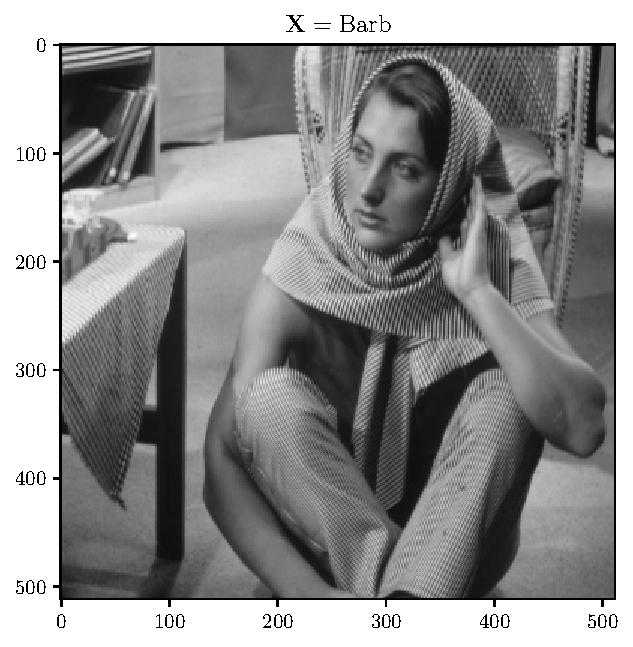
\includegraphics{barb}} & \href{https://nbviewer.org/github/vicente-gonzalez-ruiz/denoising/blob/main/figs/averaging_denoising.ipynb\#0MMPG_barb}{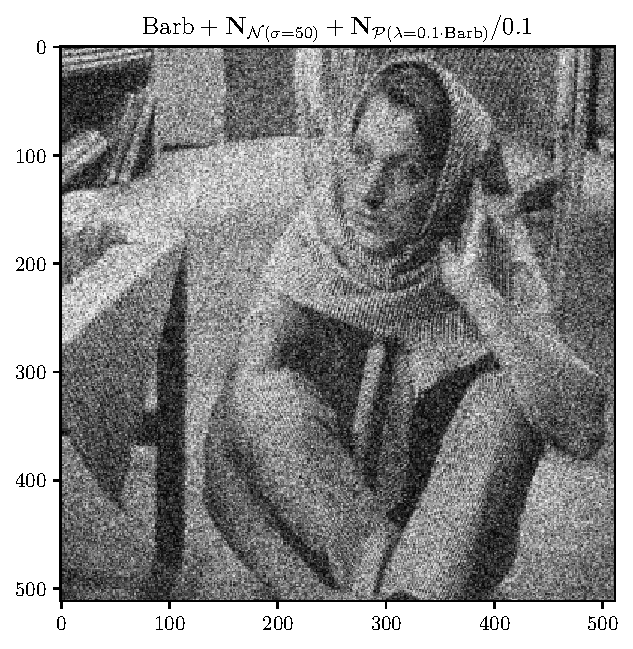
\includegraphics{0MMPG_barb}} \\
      \href{https://nbviewer.org/github/vicente-gonzalez-ruiz/denoising/blob/main/figs/averaging_denoising.ipynb\#averaging_0MMPG_barb}{\includegraphics{averaging_0MMPG_barb}} & \href{https://nbviewer.org/github/vicente-gonzalez-ruiz/denoising/blob/main/figs/averaging_denoising.ipynb\#PSNR_averaging_0MMPG_barb}{\includegraphics{PSNR_averaging_0MMPG_barb}}
    \end{tabular}
  }
  \caption{Effect of zero-mean MPG noise in an image and how averaging
    can be used to remove it. The clean image of Barb is shown on the
    top left, and a noisy version on the top right. On to bottom, the
    left image shows a denoised version after averaging, and on the right
    the graph shows the performance of the averaging process for different
    levels of noise.\label{fig:averaging_0MMPG}}
\end{figure}

\begin{comment}
Fig.~\ref{fig:0MAUN} shows an
example of how zero-mean uniform noise is cancelled by averaging.
  
  \begin{figure}
    \centering
    \resizebox{1.0\textwidth}{!}{
      \renewcommand{\arraystretch}{0.0} % Adjust row spacing in the table
      \setlength{\tabcolsep}{0ex}      % Adjust column spacing in the table    
      \begin{tabular}{cc}
        \href{https://nbviewer.org/github/vicente-gonzalez-ruiz/denoising/blob/main/figs/averaging_denoising.ipynb\#Display-Barb}{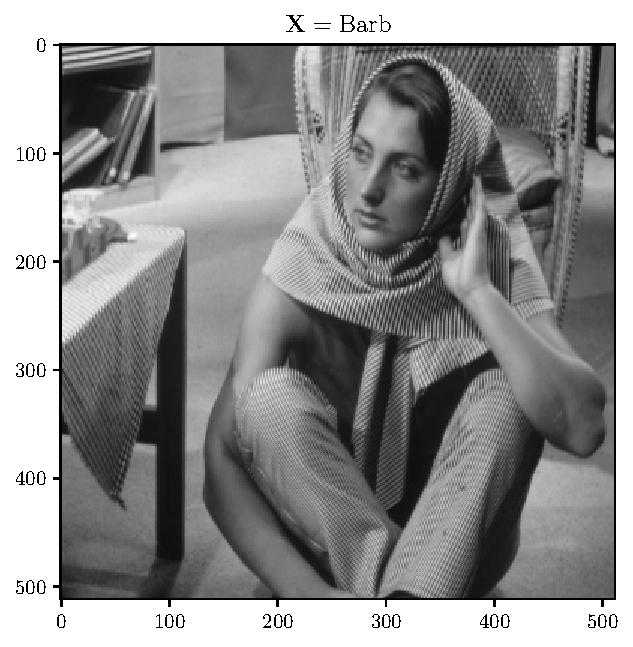
\includegraphics{barb}} & \href{https://nbviewer.org/github/vicente-gonzalez-ruiz/denoising/blob/main/figs/averaging_denoising.ipynb\#0MAUN_barb}{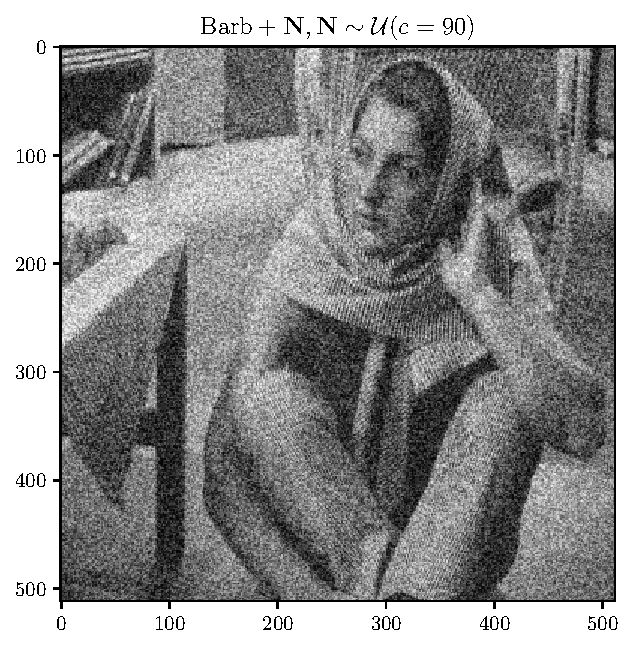
\includegraphics{0MAUN_barb}} \\
        \href{https://nbviewer.org/github/vicente-gonzalez-ruiz/denoising/blob/main/figs/averaging_denoising.ipynb\#denoised_0MAUN_barb}{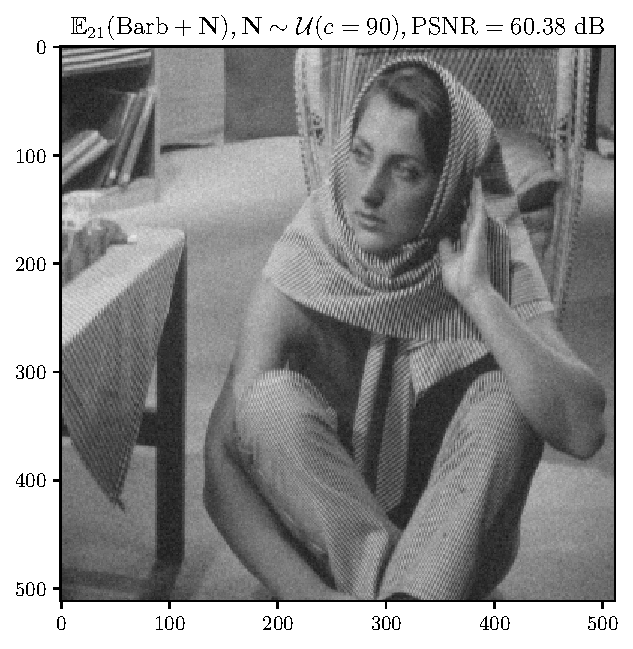
\includegraphics{denoised_0MAUN_barb}} & \href{https://nbviewer.org/github/vicente-gonzalez-ruiz/denoising/blob/main/figs/averaging_denoising.ipynb\#PSNR_0MAUN_barb}{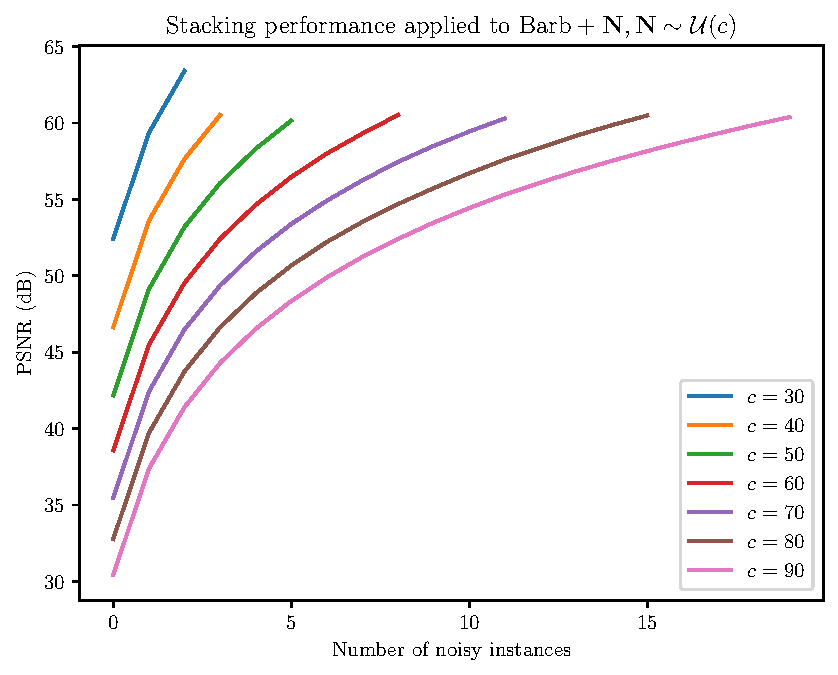
\includegraphics{PSNR_0MAUN_barb}}
      \end{tabular}
    }
    \caption{Effect of zero-mean additive uniform noise in an image
      and how averaging can be used to reduced by averaging. The clean
      image of Barb is shown on the top left, and a noisy version on
      the top right. On to bottom, the left image shows a denoised
      version after averaging and the right graph shows the performance
      of the averaging process for different levels of
      noise.\label{fig:0MAUN}}
  \end{figure}

 Fig.~\ref{fig:0MAGN} shows an
  example of how zero-mean Gaussian noise is cancelled by averaging.

  \begin{figure}
    \centering
    \resizebox{1.0\textwidth}{!}{
      \renewcommand{\arraystretch}{0.0} % Adjust row spacing in the table
      \setlength{\tabcolsep}{0ex}      % Adjust column spacing in the table    
      \begin{tabular}{cc}
        \href{https://nbviewer.org/github/vicente-gonzalez-ruiz/denoising/blob/main/figs/averaging_denoising.ipynb\#barb}{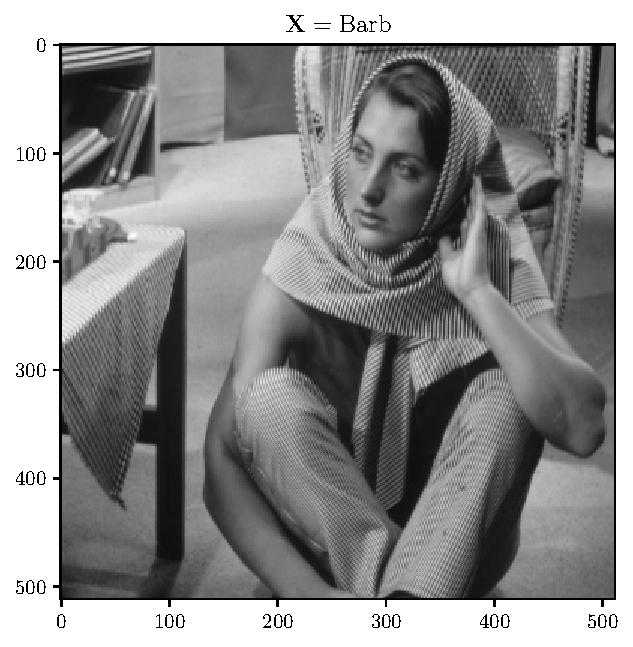
\includegraphics{barb}} & \href{https://nbviewer.org/github/vicente-gonzalez-ruiz/denoising/blob/main/figs/averaging_denoising.ipynb\#0MAGN_barb}{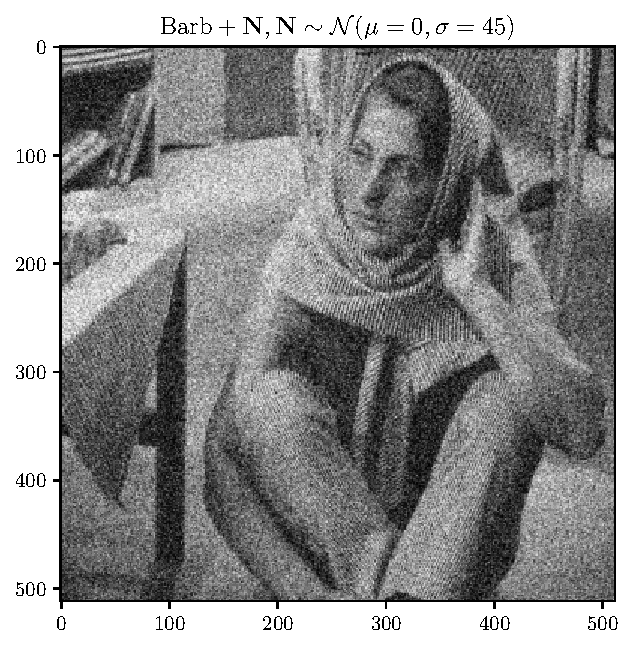
\includegraphics{0MAGN_barb}} \\
        \href{https://nbviewer.org/github/vicente-gonzalez-ruiz/denoising/blob/main/figs/averaging_denoising.ipynb\#denoised_0MAGN_barb}{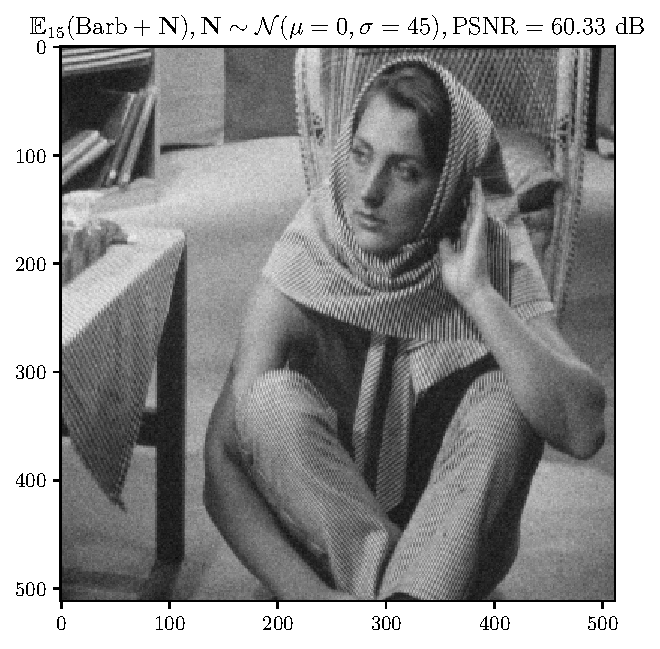
\includegraphics{denoised_0MAGN_barb}} & \href{https://nbviewer.org/github/vicente-gonzalez-ruiz/denoising/blob/main/figs/averaging_denoising.ipynb\#PSNR_0MAGN_barb}{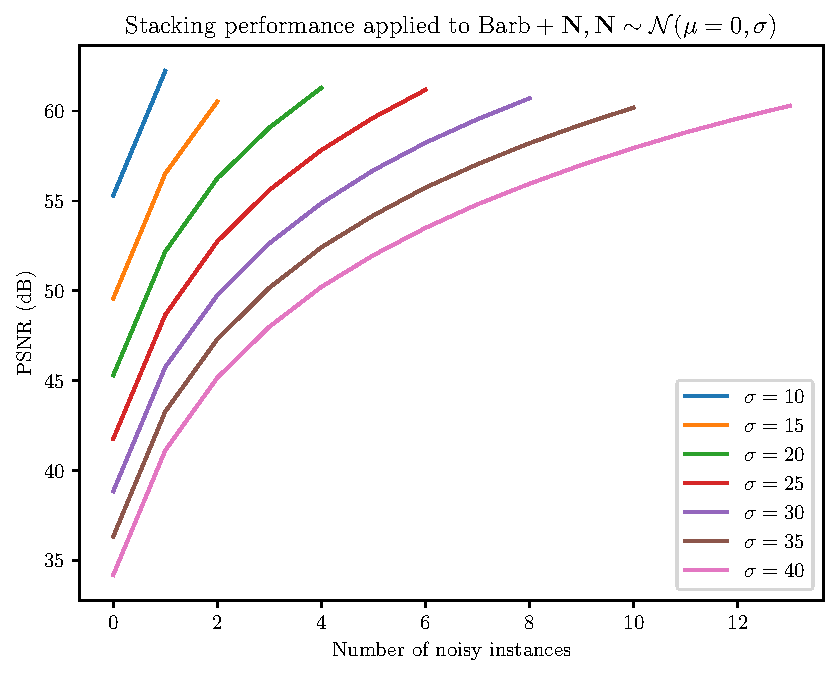
\includegraphics{PSNR_0MAGN_barb}}
      \end{tabular}
    }
    \caption{Effect of zero-mean additive Gaussian noise in an image
      and how averaging can be used to reduced by averaging. The clean
      image of Barb is shown on the top left, and a noisy version on
      the top right. On to bottom, the left image shows a denoised
      version after averaging and the right graph shows the performance
      of the averaging process for different levels of
      noise.\label{fig:0MAGN}}
  \end{figure}

  Fig.~\ref{fig:0MMGN} shows an example of
  how zero-mean Gaussian noise is cancelled by averaging.

  \begin{figure}
    \centering
    \resizebox{1.0\textwidth}{!}{
      \renewcommand{\arraystretch}{0.0} % Adjust row spacing in the table
      \setlength{\tabcolsep}{0ex}      % Adjust column spacing in the table    
      \begin{tabular}{cc}
        \href{https://nbviewer.org/github/vicente-gonzalez-ruiz/denoising/blob/main/figs/averaging_denoising.ipynb\#barb}{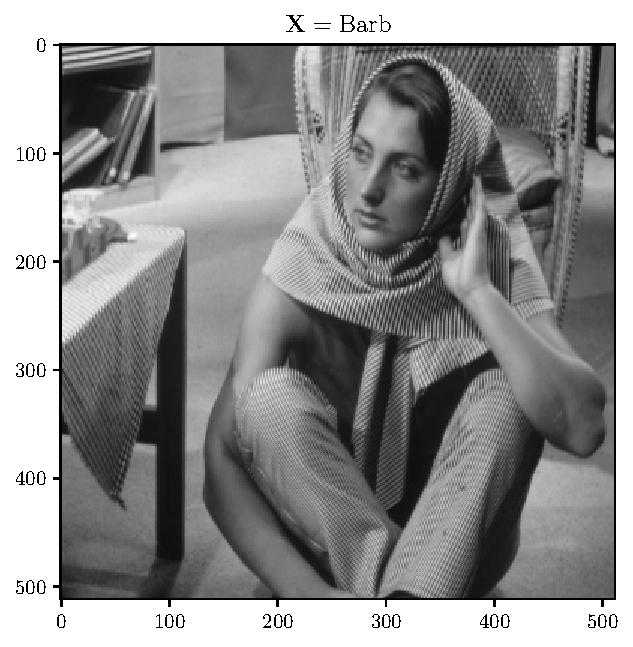
\includegraphics{barb}} & \href{https://nbviewer.org/github/vicente-gonzalez-ruiz/denoising/blob/main/figs/averaging_denoising.ipynb\#0MMGN_barb}{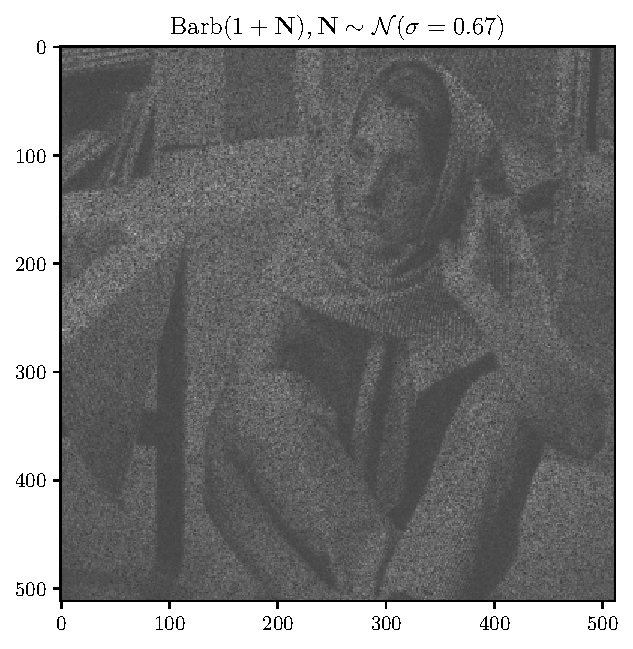
\includegraphics{0MMGN_barb}} \\
        \href{https://nbviewer.org/github/vicente-gonzalez-ruiz/denoising/blob/main/figs/averaging_denoising.ipynb\#denoised_0MMGN_barb}{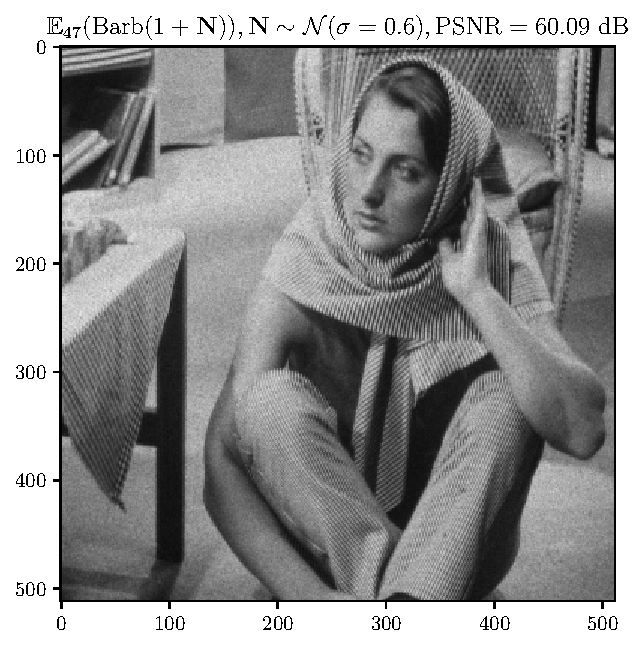
\includegraphics{denoised_0MMGN_barb}} & \href{https://nbviewer.org/github/vicente-gonzalez-ruiz/denoising/blob/main/figs/averaging_denoising.ipynb\#PSNR_0MMGN_barb}{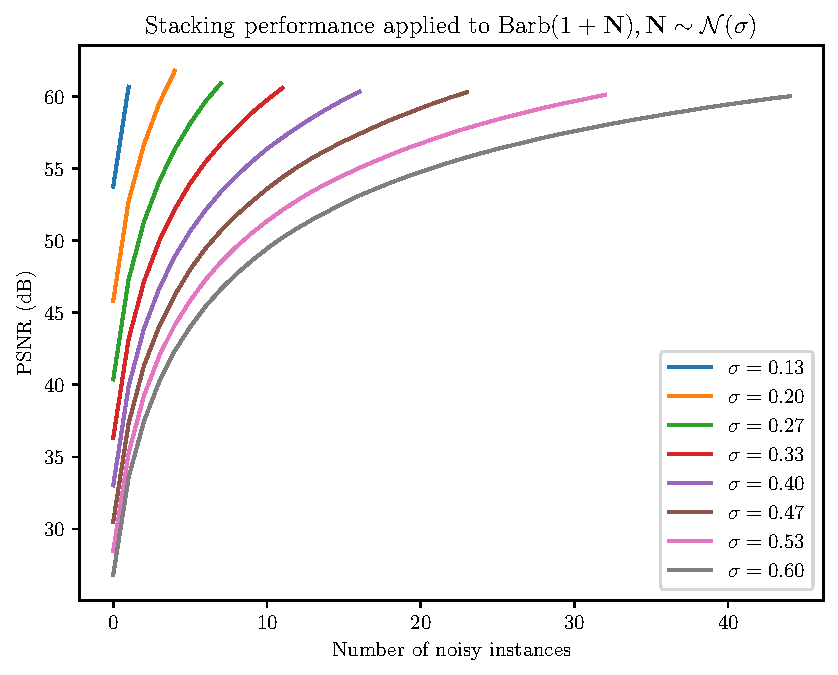
\includegraphics{PSNR_0MMGN_barb}}
      \end{tabular}
    }
    \caption{Effect of zero-mean multiplicative Gaussian noise in an
      image and how averaging can be used to reduced by averaging. The
      clean image of Barb is shown on the top left, and a noisy
      version on the top right. On to bottom, the left image shows a
      denoised version after averaging and the right graph shows the
      performance of the averaging process for different levels of
      noise.\label{fig:0MMGN}}
  \end{figure}

 Fig.~\ref{fig:Rayleigh}
  shows an example of how Rayleigh noise is cancelled by averaging.

  \begin{figure}
    \centering
    \resizebox{1.0\textwidth}{!}{
      \renewcommand{\arraystretch}{0.0} % Adjust row spacing in the table
      \setlength{\tabcolsep}{0ex}      % Adjust column spacing in the table    
      \begin{tabular}{cc}
        \href{https://nbviewer.org/github/vicente-gonzalez-ruiz/denoising/blob/main/figs/averaging_denoising.ipynb\#barb}{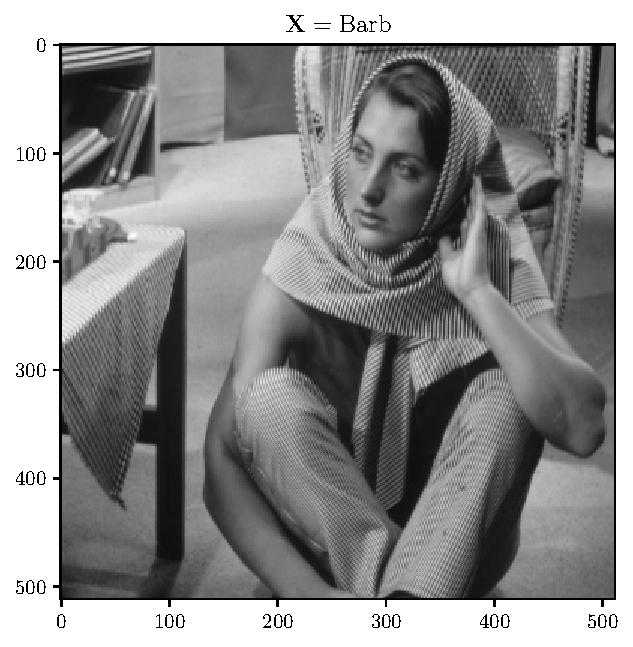
\includegraphics{barb}} & \href{https://nbviewer.org/github/vicente-gonzalez-ruiz/denoising/blob/main/figs/averaging_denoising.ipynb\#Rayleigh_barb}{\includegraphics{Rayleigh_barb}} \\
        \href{https://nbviewer.org/github/vicente-gonzalez-ruiz/denoising/blob/main/figs/averaging_denoising.ipynb\#denoised_Rayleigh_barb}{\includegraphics{denoised_Rayleigh_barb}} & \href{https://nbviewer.org/github/vicente-gonzalez-ruiz/denoising/blob/main/figs/averaging_denoising.ipynb\#PSNR_Rayleigh_barb}{\includegraphics{PSNR_Rayleigh_barb}}
      \end{tabular}
    }
    \caption{Effect of Rayleigh noise in an image and how averaging can
      be used to reduced by averaging. The clean image of Barb is shown
      on the top left, and a noisy version on the top right. On to
      bottom, the left image shows a denoised version after averaging
      and the right graph shows the performance of the averaging
      process for different levels of noise.\label{fig:Rayleigh}}
  \end{figure}

  Fig.~\ref{fig:Poisson} shows an example of how Poisson noise is
  cancelled by averaging.

  \begin{figure}
    \centering
    \resizebox{1.0\textwidth}{!}{
      \renewcommand{\arraystretch}{0.0} % Adjust row spacing in the table
      \setlength{\tabcolsep}{0ex}      % Adjust column spacing in the table    
      \begin{tabular}{cc}
        \href{https://nbviewer.org/github/vicente-gonzalez-ruiz/denoising/blob/main/figs/averaging_denoising.ipynb\#barb}{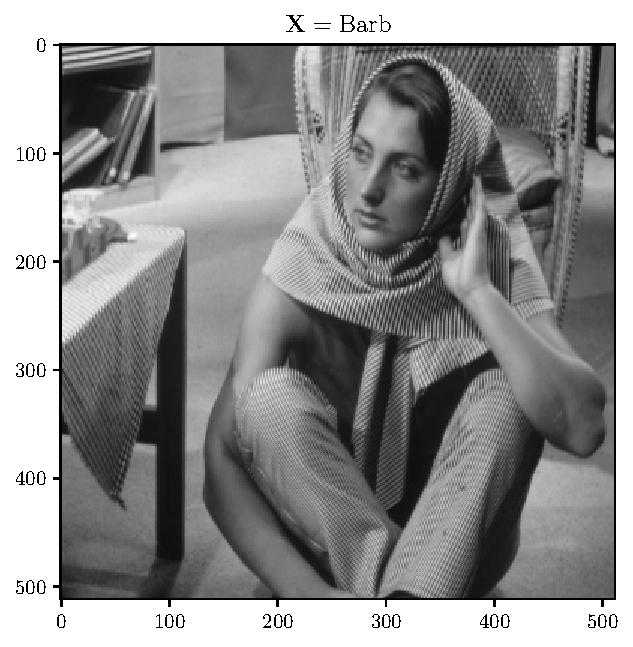
\includegraphics{barb}} & \href{https://nbviewer.org/github/vicente-gonzalez-ruiz/denoising/blob/main/figs/averaging_denoising.ipynb\#Poisson_barb}{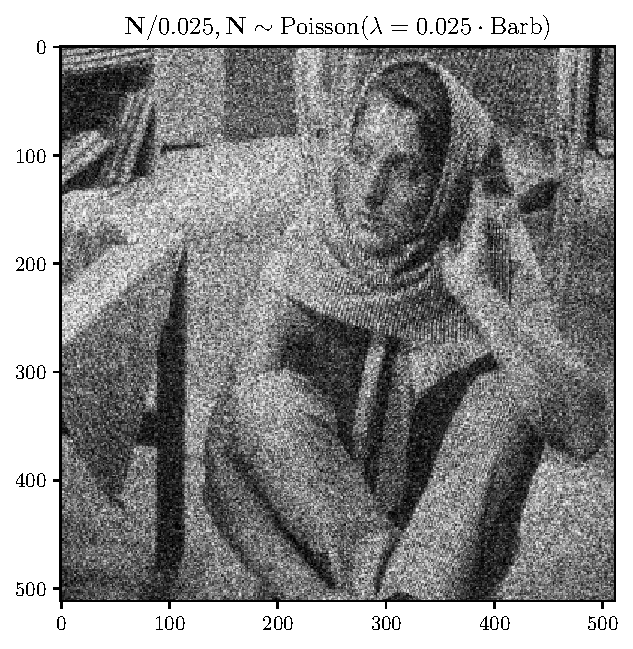
\includegraphics{Poisson_barb}} \\
        \href{https://nbviewer.org/github/vicente-gonzalez-ruiz/denoising/blob/main/figs/averaging_denoising.ipynb\#denoised_Poisson_barb}{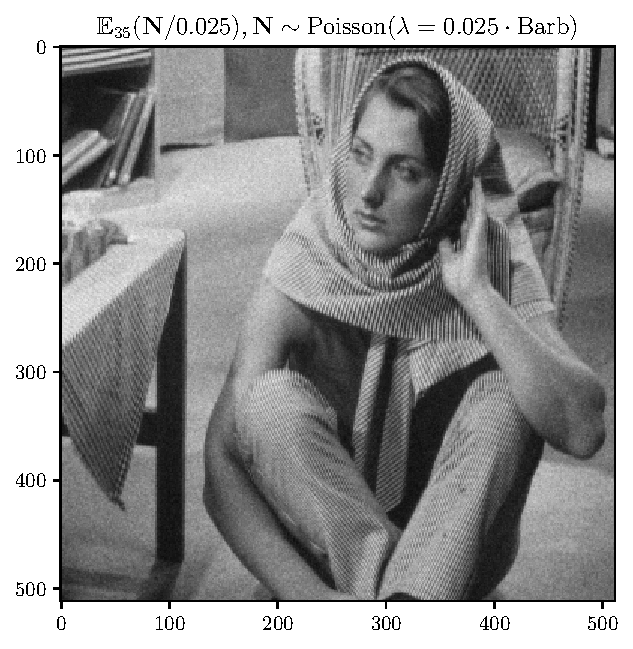
\includegraphics{denoised_Poisson_barb}} & \href{https://nbviewer.org/github/vicente-gonzalez-ruiz/denoising/blob/main/figs/averaging_denoising.ipynb\#PSNR_Poisson_barb}{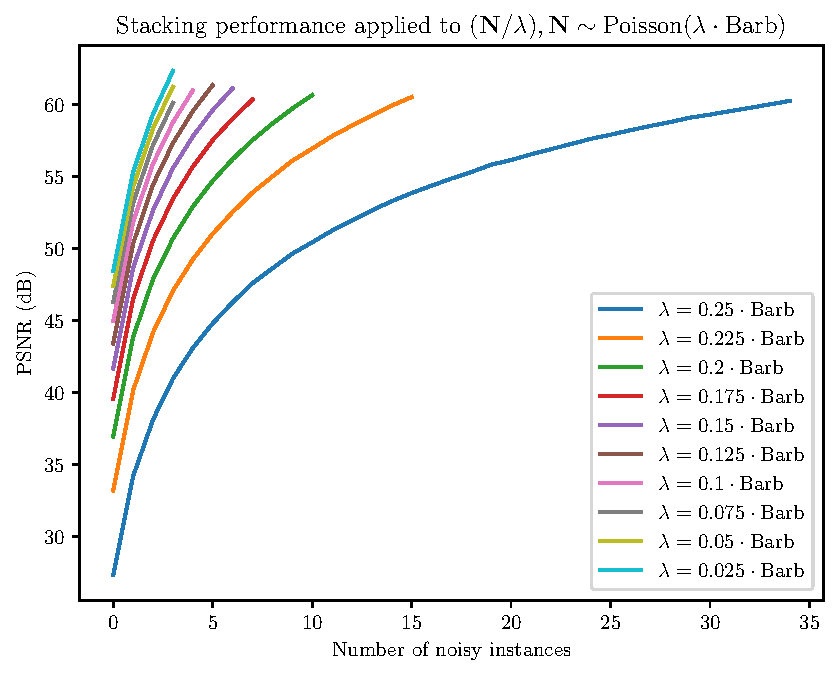
\includegraphics{PSNR_Poisson_barb}}
      \end{tabular}
    }
    \caption{Effect of Poisson noise in an image and how averaging can
      be used to reduced by averaging. The clean image is shown
      on the top left, and a noisy version on the top right. On the
      bottom, the left image shows a denoised version after averaging
      and the right graph shows the performance of the averaging
      process for different levels of noise.\label{fig:Poisson}}
  \end{figure}
\end{comment}
  
\subsection{Gaussian Denoising (GD)}

GD, also known by Gaussian smoothing filtering, works by convolving a
separable Gaussian kernel with the signal samples in each space
dimension.

1D GD can be expressed by
\begin{equation}
  \tilde{\mathbf{X}}(\Sigma) = \hat{\mathbf{Y}}*\mathbf{h}(\Sigma),
  \label{eq:GF}
\end{equation}
where $\tilde{\mathbf{X}}$ represents the denoised signal,
$\hat{\mathbf{Y}}$ the noisy instance, and $*$ the convolution of
digital (in this case, 1D) signals.

The coefficients of the Gaussian kernel
\begin{equation}
  \mathbf{h}(\Sigma) = \{\mathbf{h}_i(\Sigma)\} = \frac{1}{\sqrt{2\pi}\Sigma}e^{{-i}^2/(2\Sigma^2)},
  \label{eq:GK}
\end{equation}
defines a low-pass filter under the assumption that most of the energy
(and information) is concentrated in the low frequencies, where
$\Sigma$ is a parameter that controls the length of the kernel and
therefore, the cut-off frequency of GD (a higher $\Sigma$ results in a
lower the cut-off frequency, and therefore, in a higher smoothing
effect).

As can be seen in Eq.~\ref{eq:GK} (all the kernel coefficients are
positive), and computes weighted averages of neighbour signal
samples. This does not mach the calculus described in
Eq.~\ref{eq:averaging_result}, but as an advantage, GD requires only a
noisy instance. The result of GD is a smooth denoised signal
$\tilde{\mathbf X}$.

Multidimensional GD is separable, which means that we can apply the 1D
filter to all the dimensions of the signal to compute a $N$D
denoising. For the 3D case, we have that
\begin{equation}
  \tilde{\mathbf{X}}(\Sigma) = \Big(\big(\hat{\mathbf X}*^{(\text{Z})}{\mathbf h}(\Sigma)\big)*^{(\text{Y})}{\mathbf h}(\Sigma)\Big)*^{(\text{X})}{\mathbf h}(\Sigma),
    \label{eq:3DGF}
\end{equation}
where ${\mathbf s}*^{(d)}{\mathbf h}$ is the 1D convolution applied to
the dimension $d$ of the signal ${\mathbf s}$ and the 1D filter
${\mathbf h}$. For simplicity, Eq.~\ref{eq:3DGF} defines isotropic
filtering, but the length of the kernel can be different at each
dimension to provide anisotropic filtering.

\begin{figure}
  \centering
  \resizebox{1.0\textwidth}{!}{
    \renewcommand{\arraystretch}{0.0} % Adjust row spacing in the table
    \setlength{\tabcolsep}{0ex}      % Adjust column spacing in the table    
    \begin{tabular}{cc}
      \href{https://nbviewer.org/github/vicente-gonzalez-ruiz/denoising/blob/main/figs/averaging_denoising.ipynb\#0MMPG_barb}{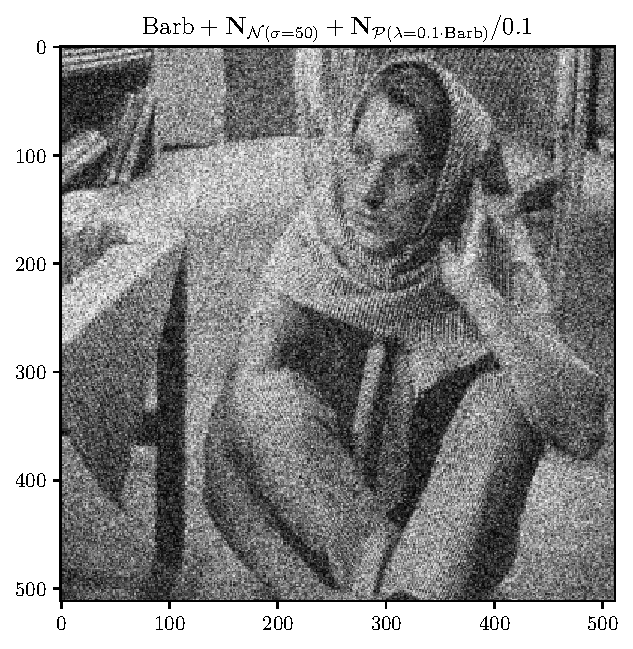
\includegraphics{0MMPG_barb}} & \href{https://nbviewer.org/github/vicente-gonzalez-ruiz/denoising/blob/main/figs/averaging_denoising.ipynb\#GD_0MMPG_barb}{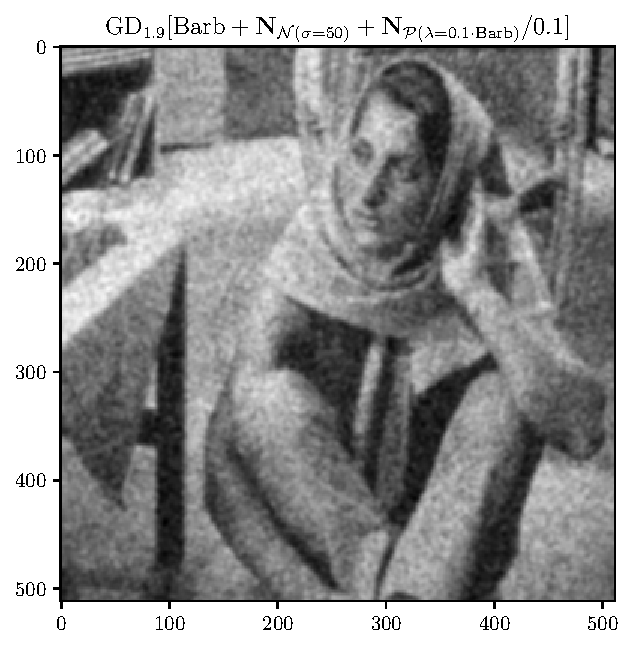
\includegraphics{GD_0MMPG_barb}} \\
      \href{https://nbviewer.org/github/vicente-gonzalez-ruiz/denoising/blob/main/figs/averaging_denoising.ipynb\#GD_PCC_0MMPG_barb}{\includegraphics{GD_PCC_0MMPG_barb}} & \href{https://nbviewer.org/github/vicente-gonzalez-ruiz/denoising/blob/main/figs/averaging_denoising.ipynb\#GD_SFRC_0MMPG_barb}{\includegraphics{GD_SFRC_0MMPG_barb}}
    \end{tabular}
  }
  \caption{Effect of zero-mean MPG noise in an image and how Gaussian
    denoising (GD) can be used to reduce it. A noisy version of the
    image is on the top left. On the right, a denoised version using
    Gaussian denoising. On the bottom left it is shown the performance
    of GD for different levels of noise. On the right, the SFRC of one
    of a denoised image.\label{fig:GD_0MMPG}}
\end{figure}

Fig.~\ref{fig:GD_0MMPG} shows the performance of GD in a artificially
noised image, for different levels of noise. As can be seen, the
optimal value for the single parameter that GD requires (the length of
the Gaussian kernels in each dimension) depends on the noise level, an
information that is generally unknown in microscopy imaging.

For this reason, the autocorrelation in the Fourier domain has been
calculated by subbands of a filtered image, generating a number of
SFRC curves, one for each different kernel length $\Sigma$. As can be
seen, the autocorrelation increases when the noise level decreases due
to increasing $\Sigma$, until it reaches a value for which the
autocorrelation decreases again. For that $\Sigma^*$, which maximizes
the area under the curve up to the normalized frequency $\omega/2$, is
when the PCC metric is also maximized (for $\Sigma^*/2$), which means
that we can use the SFRC metric (in the 2D case) and the SFSC (in the
3D case) to optimize the filtering parameters.

\subsection{SDPG (Structure-Preserving Gaussian Denoising) \cite{gonzalez2023structure}}

SDPG is based in 3D Gaussian filtering (Eq.~\ref{eq:3DGF}), but the noised
volume ${\mathbf Y}$ is dynamically warped to decrease the bluring at the
structures detected by an 2-D OF (Optical Flow) estimator:
\begin{equation}
  \hat{\mathbf{Y}}(\sigma; w, l) = \Big(\big(R_\text{Z}(\mathbf{Y}; w, l)*^{(\text{Z})}{\mathbf h}(\sigma)\big)*^{(\text{Y})}{\mathbf h}(\sigma)\Big)*^{(\text{X})}{\mathbf h}(\sigma),
    \label{eq:SDPG}
\end{equation}
where
\begin{equation*}
    \begin{array}{rclll}
    R_\text{Z}(\mathbf{Y}; w, l) & = & \big\{ \{ \overset{z'\rightarrow z}{\mathbf d}({\mathbf Y}_{[z',:,:]}; w, l)~:~\overset{z'\rightarrow z}{\mathbf d}({\mathbf Y}_{[z',:,:]})\approx{\mathbf Y}_{[z,:,:]} & \\ & & \text{for}
 ~z'=z-k,\cdots,z+k\} ~\text{for}~z=0,1,\cdots,N_\text{Z}-1\big\}, \\
    R_\text{Y}(\mathbf{Y}; w, l) & = & \big\{ \{ \overset{y'\rightarrow y}{\mathbf d}({\mathbf Y}_{[:,y',:]}; w, l)~:~\overset{y'\rightarrow y}{\mathbf d}({\mathbf Y}_{[:,y',:]}; w, l)\approx{\mathbf Y}_{[:,y,:]} & \\ & & \text{for}
 ~y'=y-k,\cdots,y+k\} ~\text{for}~y=0,1,\cdots,N_\text{Y}-1\big\},~\text{and} \\
    R_\text{X}(\mathbf{Y}; w, l) & = & \big\{ \{ \overset{x'\rightarrow x}{\mathbf d}({\mathbf Y}_{[:,:,x']}; w, l)~:~\overset{x'\rightarrow x}{\mathbf d}({\mathbf Y}_{[:,:,x']}; w, l)\approx{\mathbf Y}_{[:,:,x]} & \\ & & \text{for}
 ~x'=x-k,\cdots,x+k\} ~\text{for}~x=0,1,\cdots,N_\text{X}-1\big\}
    \end{array}
\end{equation*}
are the warped volumes. For example,
$\overset{x'\rightarrow x}{\mathbf d}({\mathbf Y}_{[:,:,x']}; w, l)$
represents the projection of the slice at coordinate $x'$ fulfilling
that
$\overset{x'\rightarrow x}{\mathbf d}({\mathbf Y}_{[:,:,x']}; w,
l)\approx{\mathbf Y}_{[:,:,x]}$. Notice that, for each possible offset
in ${\mathbf Z}$, ${\mathbf Y}$, and ${\mathbf X}$, a different set of
warped 2-D slices must be computed.

As indicated in Eq.~\ref{eq:SDPG}, the estimator requires 2 new
parameters:
\begin{enumerate}
\item $w$, the size of a 2D window used to analyze the 2D slices. If
  $w$ is large, the estimator is less sensitive to the noise but also
  the small structures are ignored. Therefore, higher $w$ values
  increases blurring.
\item $l$, that controls the maximun displacements that the
  estimator can generate. Blurring increases with $l$.
\end{enumerate}


% \section{AND}

% \section{N2V}
% A. Krull, T.-O. Buchholz, and F. Jug, “Noise2void-learning denoising
% from single noisy images,” in Proceedings of the IEEE/CVF conference
% on computer vision and pattern recognition, 2019, pp. 2129–2137.



\subsection{Cryo-CARE \cite{buchholz2019cryo}}
CARE (Content-Aware image REstoration) methods leverage
available knowledge about the data at hand ought to yield superior
restoration results \cite{weigert2018content}. Concretely, Cryo-CARE
is an implementation of Noise2Noise (N2N) \cite{lehtinen2018noise2noise}.

N2N is a ``supervised'' learning method for denoising where the model
(a U-Net) is trained on pairs of noisy images. However, unlike
clasical supervised denoising deep-learning based models, that
implement
\begin{equation}
  \underset{\theta}{\operatorname{arg\,min}} \, \sum_j L \big(f_\theta(\hat{\mathbf X}_j^{(1)}), {\mathbf X}_j\big)
\end{equation}
where $\{(\hat{\mathbf X}_j^{(1)}, {\mathbf X}_j)\}_{j=1}^M$ is the training
dataset, and $L$ is a given lost function such as the MSE (here higher
values mean worst results), N2N solves
\begin{equation}
  \underset{\theta}{\operatorname{arg\,min}} \, \sum_j L \big(f_\theta(\hat{\mathbf X}_j^{(1)}), {\mathbf X}_j^{(2)}\big).
\end{equation}
In other words, given two noisy versions
$\{\hat{\mathbf Y}^{(1)}, \hat{\mathbf Y}^{(2)}\}$ of the same (clean)
volume ${\mathbf Y}$, N2N learns to infeer a denoised volume
\begin{equation}
  \tilde{\mathbf Y}=\frac{1}{2}\big(f_\theta(\hat{\mathbf Y}^{(1)})+f_\theta(\hat{\mathbf Y}^{(2)})\big)\approx{\mathbf Y}.
\end{equation}
Obviously, better approximations to ${\mathbf Y}$ will be obtained
having more noisy instances, after averaing all the denoised volumes.

\subsection{NLM (Non Local Means)} 

\subsection{BM4D}

\subsection{2D-RSVD (2D Random Shuffing Volume Denoising}

\subsection{3D-RSVD (3D Random Shuffling Volume Denoising}


\bibliographystyle{plain}
\bibliography{signal_processing,microscopy,denoising}

\end{document}
